\chapter{数据分析}
\section{辐射通量密度与辐射收支}
测站测量的辐射分为长波辐射和短波辐射。
短波辐射通量密度由辐射仪观测,有向下、向上两个分量,分别记为 \(R_{s}\downarrow\),\(R_{s}\uparrow\)。
太阳辐射传播到地球,
一部分穿过大气层直接射到地面为直接太阳辐射;另外一部分被大气层中的水汽、二氧化碳、颗粒物等散射、吸收、反射,
被散射的太阳辐射一部分方向向上远离地面,一部分方向向下到达地面,到达地面的这部分为散射太阳辐射。
向下短波辐射包括直接太阳辐射和散射太阳辐射,向上短波辐射主要是地面反射的短波辐射。
长波辐射也有向下、向上两个分量,分别记作 \(R_{l}\downarrow\),\(R_{l}\uparrow\) 。
大气释放长波辐射,一部分向下到达地面被测站接收,这部分为向下长波辐射,
地面也会释放向上的长波辐射,这部分构成向上长波辐射。\cite{tagkey2006}
向下辐射通量密度与向上辐射通量密度的差值构成测站接收的净辐射通量密度,记作 \(R_n\),即:
\begin{equation}\label{eq:Rn}
  R_n = R_{s}\downarrow - R_{s}\uparrow + R_{l}\downarrow - R_{l}\uparrow
\end{equation}

2016 年 4 月 26 日至 2016 年 4 月 30 日的向下短波辐射通量密度如图\ref{fig:20160426_20160430_DSR},
白天有太阳辐射,向下短波辐射通量密度大于 0,夜晚降为 0。
这 5 天里,前两天是阴天,后两天是晴天,晴天里科大站和科学岛站的向下短波辐射通量密度的观测值与理论值非常接近,
误差平均不超过只有 16.5 $W/m^{2}$,晴天的向下短波辐射通量密度在正午达到峰值。
\begin{figure}[H]
\centering
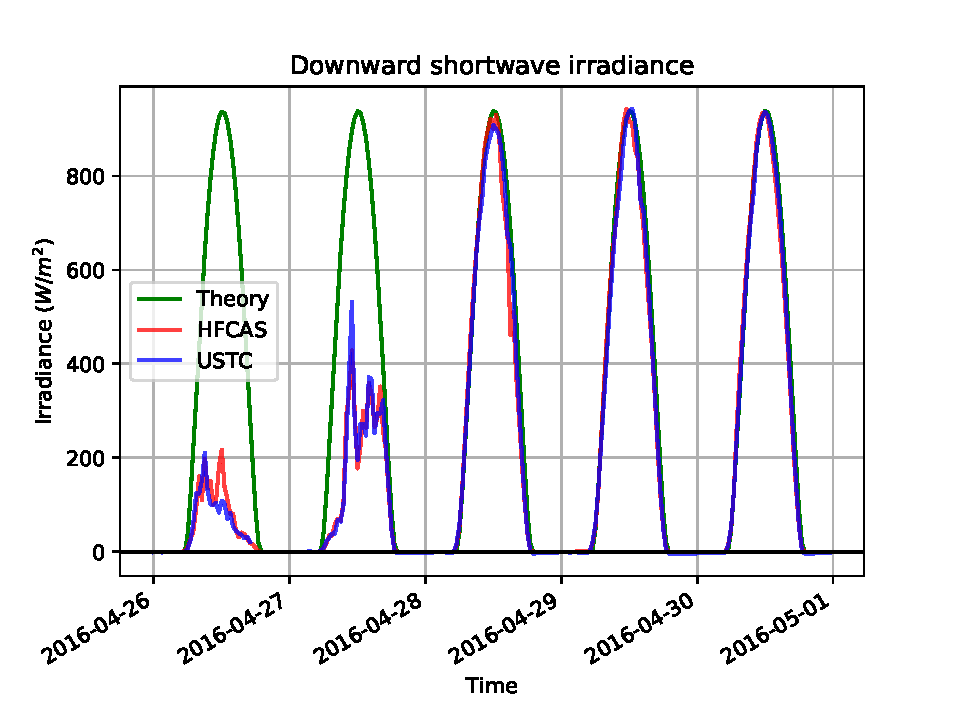
\includegraphics[width=.9\linewidth]{20160426_20160430_DSR}
\caption{2016 年 4 月 26 日至 2016 年 4 月 30 日向下短波辐射通量密度}\label{fig:20160426_20160430_DSR}\note{图中绿色表示向下短波辐射通量密度的理论值,红色表示科学岛站观测的向下短波辐射通量密度,蓝色表示中科大站观测的向下短波辐射通量密度。4 月 26 日、27 日阴天,接下来 3 天是晴天。}
\end{figure}
2016 年 4 月 26 日至 2016 年 4 月 30 日向上短波辐射通量密度如图\ref{fig:20160426_20160430_USR}
\begin{figure}[H]
\centering
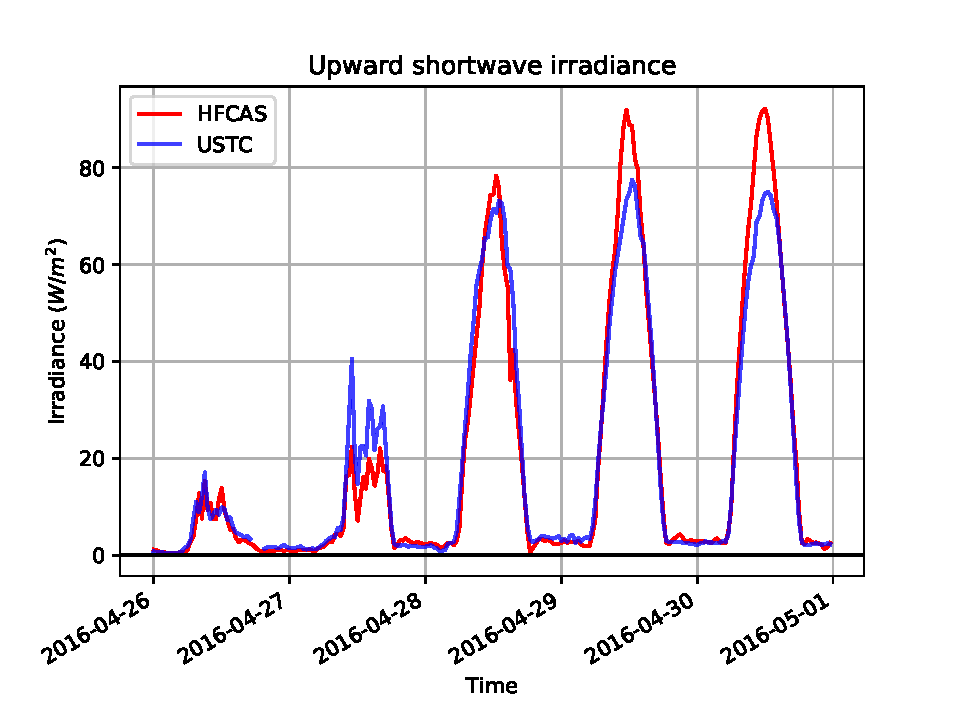
\includegraphics[width=.9\linewidth]{20160426_20160430_USR}
\caption{2016 年 4 月 26 日至 2016 年 4 月 30 日向上短波辐射通量密度}\label{fig:20160426_20160430_USR}\note{红色表示科学岛站观测的向上短波辐射通量密度,蓝色表示中科大站观测的向上短波辐射通量密度。}
\end{figure}
向上短波辐射通量密度与向下短波辐射通量密度的变化趋势保持一致。
4 月 26 日、27 日是阴天,总辐射较少,相应的向上反射的短波辐射也比较弱;后三天是晴天,总辐射强,
相应的向上反射的短波辐射也比较强,在正午达到峰值。夜间向上短波辐射通量密度平均为 3 $W/m^{2}$,
不为零的现象可能与人类活动有关,夜晚建筑和路灯的灯光会辐射出一定的短波辐射。同时注意到晴天里,
科学岛站的向上短波辐射通量密度较高,分析反照率,如图\ref{fig:20160426_20160430_albedo},
4 月 29 日正午和 4 月 30 日正午,与科大站相比科学岛站的反照率分别高出 0.017 和 0.019,
向上短波辐射通量密度分别高出 14.17 $W/m^{2}$ 和 17.45 $W/m^{2}$,这可能与测站下垫面的材质有关,
科大站在楼顶,下方铺有黑色防水油毡纸,对太阳光的吸收能力更强,
科学岛站塔下为绿色草坪,对太阳光的反射能力更强。
\begin{figure}[H]
\centering
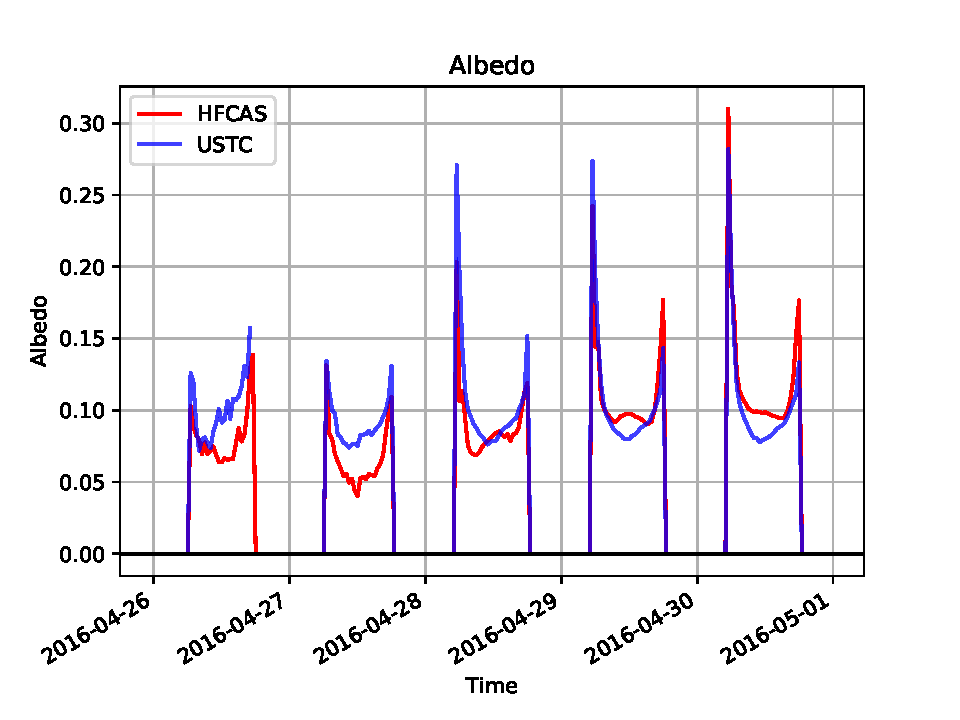
\includegraphics[width=.9\linewidth]{20160426_20160430_albedo}
\caption{2016 年 4 月 26 日至 2016 年 4 月 30 日反照率}\label{fig:20160426_20160430_albedo}
\note{红色表示科学岛站观测的反照率,蓝色表示中科大站观测的反照率。}
\end{figure}

下面再来看长波辐射,首先分析 2016 年 1 月 21 日至 2016 年 1 月 26 日两地的向下长波辐射,
如图\ref{fig:20160121_20160126_DLR},这 6 天里,前两天是阴天,后两天是晴天,
两地的相对湿度如图\ref{fig:20160121_20160126_RH_high},阴天时相对湿度较高,平均为 83\%,
之后天气转晴,相对湿度降到 60\% 以下,并且向下长波辐射通量密度变化趋势与相对湿度的变化趋势符合的比较好,
在 1 月 23、24、25 日这三天晴天里,科学岛站的向下长波辐射通量密度高于中科大站,
同样这三天科学岛站的相对湿度也比较高,
向下长波辐射由测站上空大气释放,水汽对向下长波辐射的影响较大。
\begin{figure}[H]
\centering
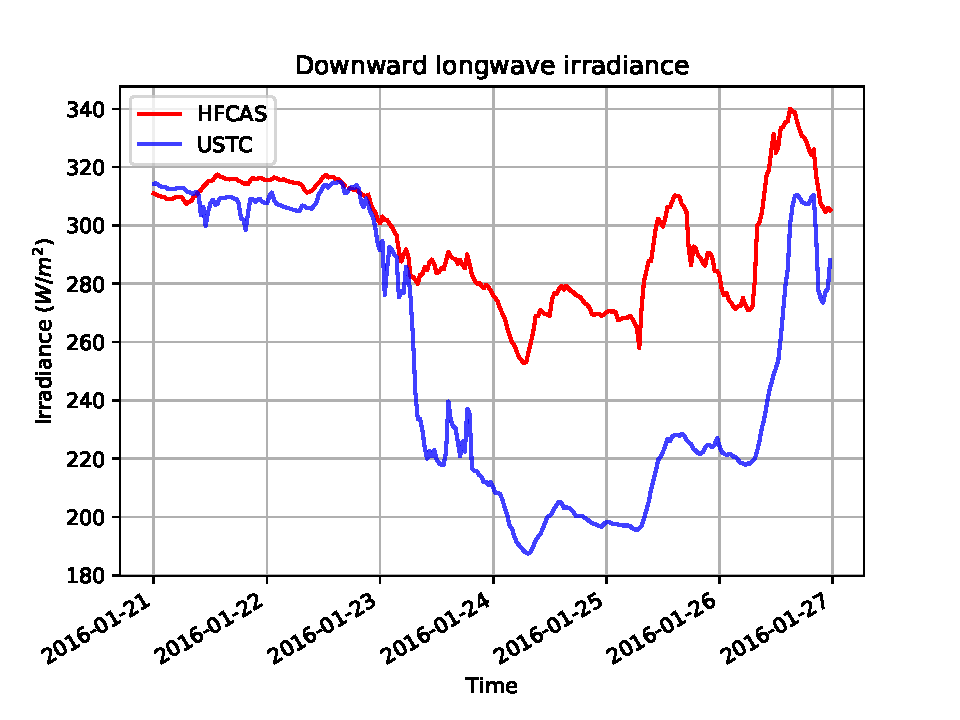
\includegraphics[width=.9\linewidth]{20160121_20160126_DLR}
\caption{2016 年 1 月 21 日至 2016 年 1 月 26 日中科大站与科学岛站两地向下长波辐射通量密度}\label{fig:20160121_20160126_DLR}
\note{图中红色表示科学岛站测得的向下长波辐射通量密度,蓝色表示中科大站观测的向下长波辐射通量密度。}
\end{figure}
\begin{figure}[H]
\centering
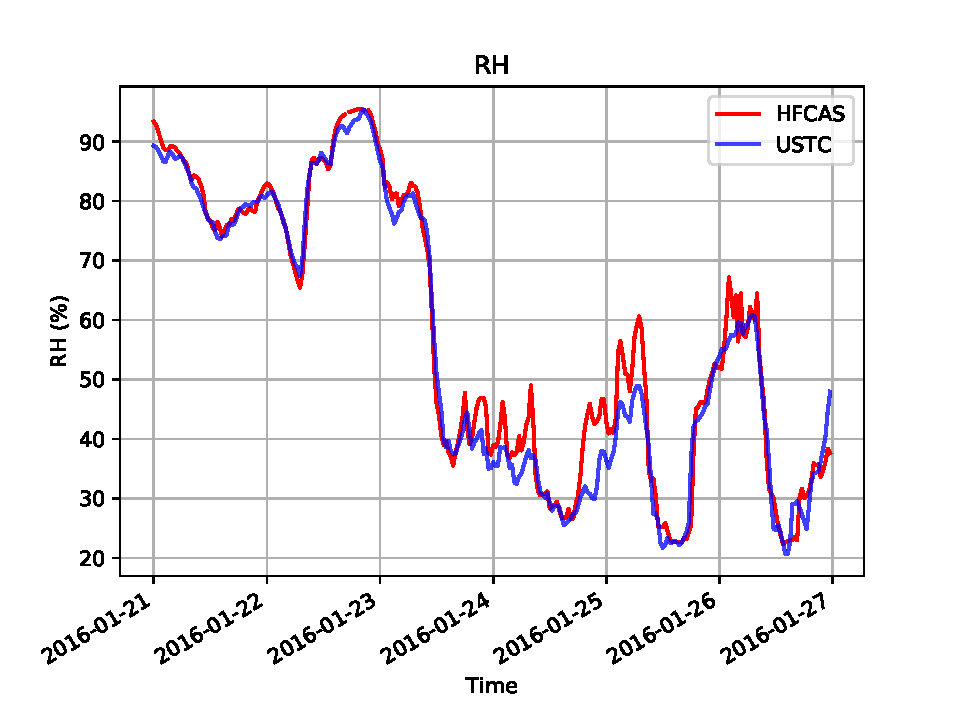
\includegraphics[width=.9\linewidth]{20160121_20160126_RH_high}
\caption{2016 年 1 月 21 日至 2016 年 1 月 26 日中科大站与科学岛站两地的相对湿度}\label{fig:20160121_20160126_RH_high}
\note{图中红色表示科学岛站测得的相对湿度,蓝色表示中科大站观测的相对湿度。}
\end{figure}

关于向上长波辐射,以 2016 年 4 月 26 日至 2016 年 4 月 30 日的向上长波辐射通量密度为例,
如图\ref{fig:20160426_20160430_ULR}
向上长波辐射由地面以及仪器下方的一部分大气向上辐射,主要反映了地面附近的温度变化。
中科大站和科学岛站向上长波辐射通量密度平均值分别为 384.68\(W/m^2\) 和 371.21\(W/m^2\),
中科大站比科学岛站高出 12.46\(W/m^2\),
晴天白天中科大站和科学岛站的向上长波辐射通量密度平均值分别为 436.70\(W/m^2\) 和 416.11\(W/m^2\),
中科大高出 20.60\(W/m^2\)。
中科大站与科学岛站晴天白天的平均温度分别为 \(16.54^{\circ}C\) 和 \(15.55^{\circ}C\),
中科大站高出 \(0.99^{\circ}C\)。
2016 年 4 月 26 日至 2016 年 4 月 30 日中科大站与科学岛站两地向上长波辐射通量密度与温度的关系如图\ref{fig:20160426_20160430_Rl_Ta},
由于没有地面温度的观测数据,只能使用观测塔最低层的数据近似作为地面温度,图中向上长波辐射通量密度与温度存在一个相位差,这个时间差可能是由地面与大气的热量交换过程导致的。
\begin{figure}[H]
\centering
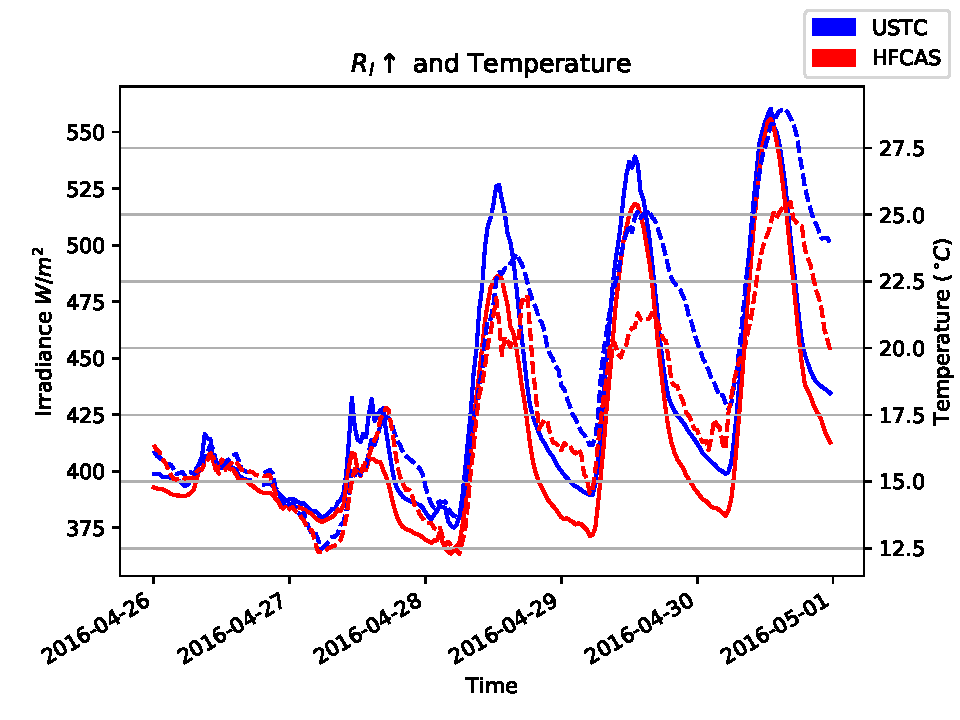
\includegraphics[width=.9\linewidth]{20160426_20160430_Rl_Ta}
\caption{2016 年 4 月 26 日至 2016 年 4 月 30 日中科大站与科学岛站两地向上长波辐射通量密度与温度}\label{fig:20160426_20160430_Rl_Ta}
\note{图中蓝色实线表示中科大站的向上长波辐射通量密度,蓝色虚线表示中科大站测量的最低层温度,红色实线表示科学岛站的向上长波辐射通量密度,红色虚线表示科学岛站测量的最低层温度。}
\end{figure}

事实上,黑体辐射与温度的关系有 Stefan-Boltzmann 定律:
\begin{equation}
  F = \sigma T^4
\end{equation}
其中,\(F\) 为辐射通量密度,\(\sigma\) 为 Stefan-Boltzmann 常数 \(5.67\times10^{-8}Wm^{-2}K^{-4}\),
\(T\) 为温度。理论上我们可以利用 Stefan-Boltzmann 定律和地面的温度数据计算出向上的长波辐射通量密度,
如图\ref{fig:20151201_20151231_ULR_Theory_HFCAS}为
2015 年 12 月科学岛站向上长波辐射通量密度的观测值与通过 Stefan-Boltzmann 定律和温度计算的理论值比较,
可以看出两者符合的比较好,经过对全部数据的分析,科大站向上长波辐射通量密度平均值为 384.68\(W/m^2\),
科学岛站向上长波辐射通量密度平均值为 371.21\(W/m^2\),
而科大站向上长波辐射通量密度的观测值与理论值平均相差 7.36\(W/m^2\),
科学岛站向上长波辐射通量密度的观测值与理论值平均相差 -2.58\(W/m^2\),
两地的观测值与理论值之差均不超过观测值的 2\%。
\begin{figure}[H]
\centering
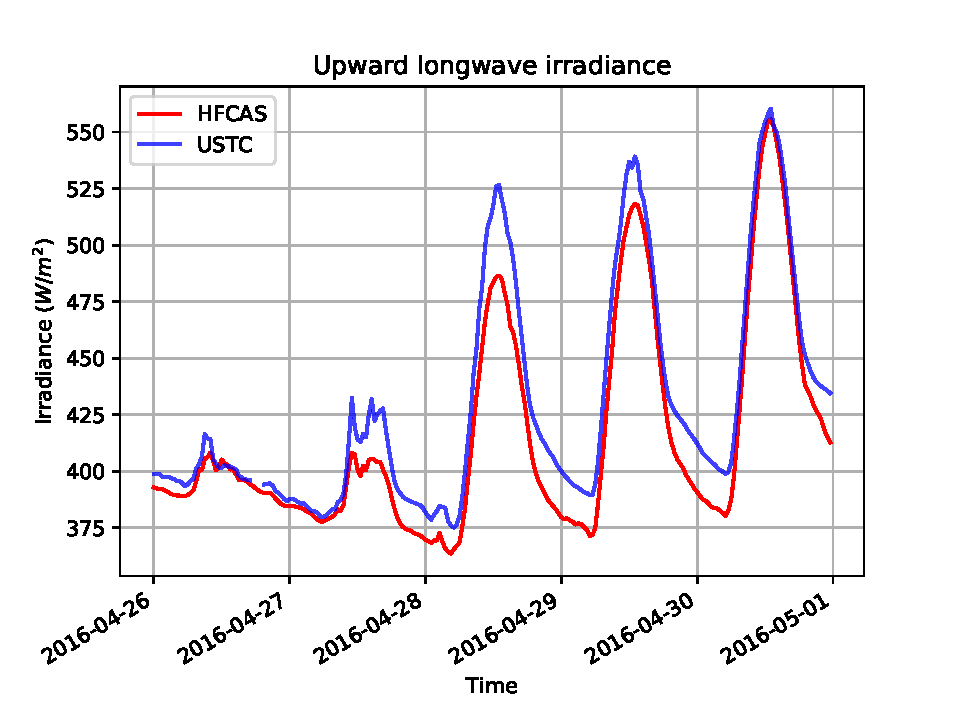
\includegraphics[width=.9\linewidth]{20160426_20160430_ULR}
\caption{2016 年 4 月 26 日至 2016 年 4 月 30 日向上长波辐射通量密度}\label{fig:20160426_20160430_ULR}
\note{红色表示科学岛站观测的向上长波辐射通量密度,蓝色表示中科大站观测的向上长波辐射通量密度。}
\end{figure}
\begin{figure}[H]
\centering
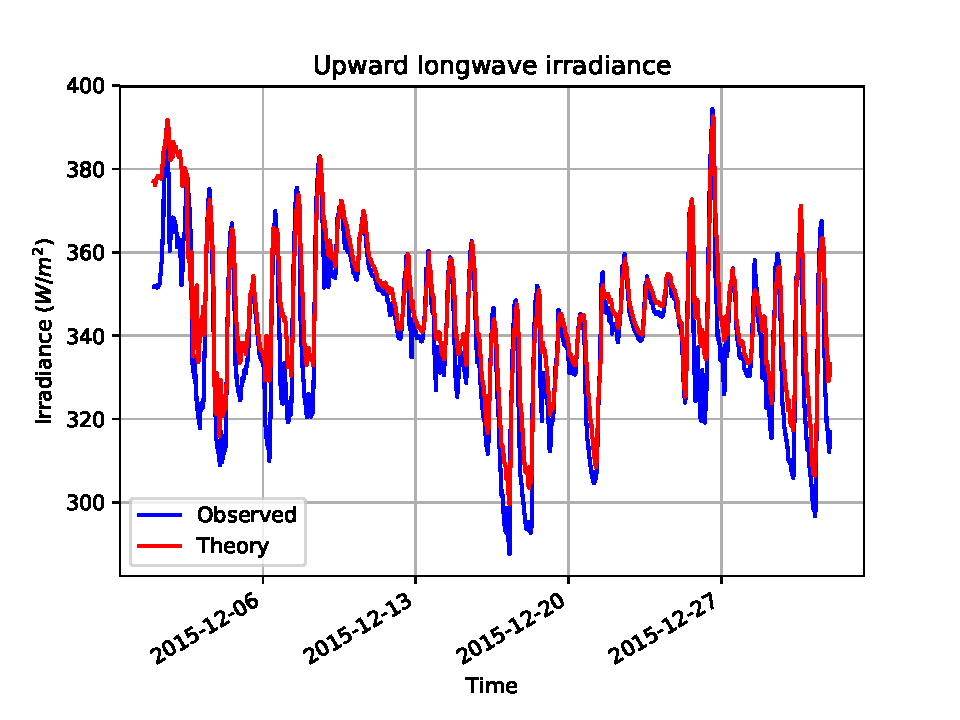
\includegraphics[width=.9\linewidth]{20151201_20151231_ULR_Theory_HFCAS}
\caption{2015 年 12 月科学岛站向上长波辐射通量密度的观测值与通过 Stefan-Boltzmann 定律和温度计算的理论值比较}\label{fig:20151201_20151231_ULR_Theory_HFCAS}
\note{图中,蓝色为辐射仪观测的向上长波辐射通量密度,红色为利用 Stefan-Boltzmann 定律和温度计算计算得到的向上长波辐射的理论值}
\end{figure}
无论是向上长波辐射通量密度还是温度,中科大站(城市)普遍都要高于科学岛站(郊区),
这体现了合肥市的城市热岛效应。城市里存在大量的建筑、沥青街道等对太阳光的吸收能力强,反照率低,
而郊区里绿色的植被、农作物等对太阳光的吸收能力较弱,反照率高,
这样,与郊区相比,城市吸收了更多的太阳辐射;
城市内建筑、街道等可能会改变自然原有的物理化学性质;
绿色植物的光合作用可以吸收二氧化碳,而城市中植被覆盖率比较低,
人们生产生活又会时刻释放出的二氧化碳,使得城市的温室效应比郊区更加严重。
此外还有很多因素可能对城市热岛效应产生影响,这些因素共同作用,
使得城市地面的温度高于郊区,释放出更强的向上长波辐射。

有了向下、向上短波辐射通量密度以及向下、向上长波辐射通量密度这 4 个分量的辐射数据之后,
便可根据式\ref{eq:Rn}计算出净辐射通量密度 \(R_n\),将观测的数据每半个月做平均得到图\ref{fig:sms_R},
图中显示了向下、向上短波辐射通量密度,向下、向上长波辐射通量密度,向下短波辐射通量密度理论值,
以及净辐射通量密度的变化趋势。
\begin{figure}[H]
\centering
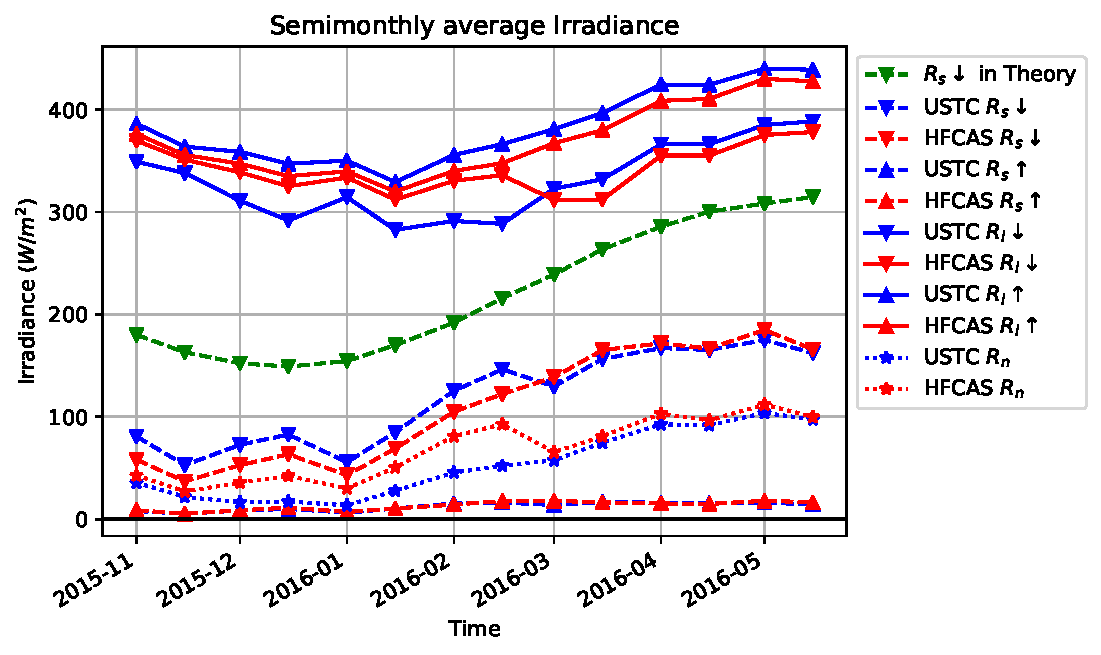
\includegraphics[width=.9\linewidth]{sms_R}
\caption{2015 年 11 月至 2016 年 5 月半月平均辐射通量密度}\label{fig:sms_R}
\note{图中,绿色代表理论值,蓝色代表中科大站,红色代表科学岛站,实线表示长波辐射通量密度,虚线表示短波辐射通量密度,点线表示净辐射通量密度,向下三角表示方向向下,向上三角表示方向向上,五角星表示方向向下的净辐射通量密度。例如:图中向上三角的蓝色实线表示中科大站观测的向上长波辐射通量密度。}
\end{figure}

\section{感热通量密度}
感热又称显热,是指物体在不发生相变的加热或冷却过程中所吸收或放出的热。
感热通量密度(Hs)描述了由于温度的变化导致的大气与下垫面之间发生的湍流热交换。\cite{tagkey2006}
2015 年 11 月至 2016 年 6 月中科大站与科学岛站的感热通量密度如图\ref{fig:Hs},
可以明显看出中科大站的感热通量密度(蓝色)普遍比科学岛站的感热通量密度(红色)要高,
具体可见表\ref{tab:Hs}。
\begin{figure}[H]
\centering
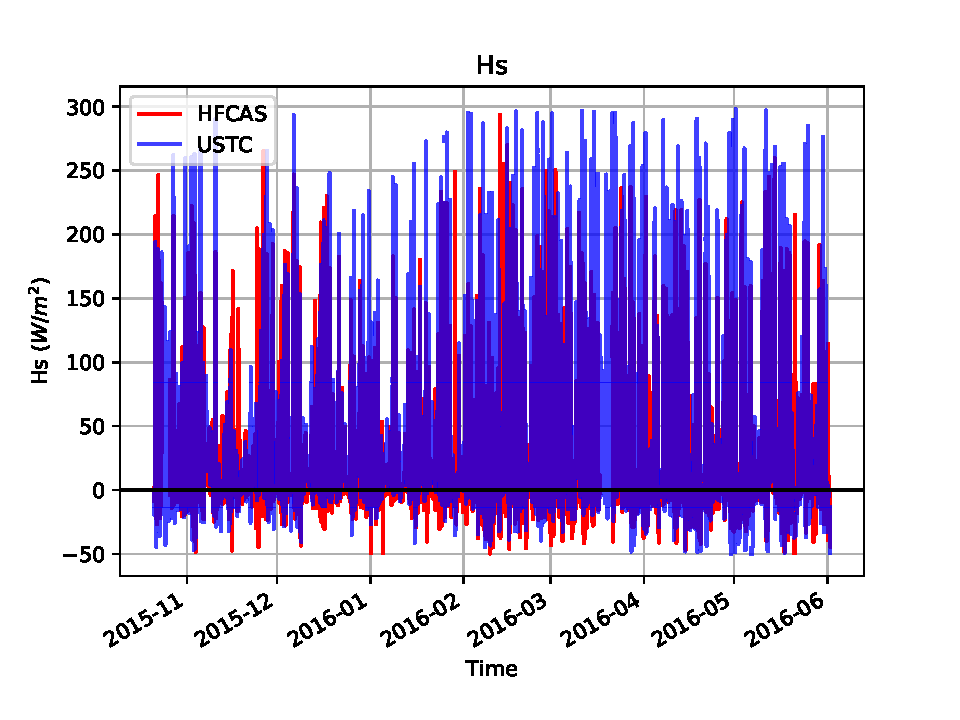
\includegraphics[width=.9\linewidth]{Hs}
\caption{2015 年 11 月至 2016 年 6 月感热通量密度}\label{fig:Hs}
\note{红色表示科学岛站观测的感热通量密度,蓝色表示中科大站观测的感热通量密度。}
\end{figure}

\begin{table}[H]
\centering
\caption{中科大站与科学岛站感热通量密度比较}\label{tab:Hs}
\begin{tabular}{ccccc}
  \toprule
  & \multicolumn{2}{c}{中科大站} & \multicolumn{2}{c}{科学岛站}\\
  \cmidrule(r){2-3} \cmidrule(r){4-5}
  & 均值 & 标准差 & 均值 & 标准差\\
  \midrule
  全部 & 30.391 & 60.838 & 19.677 & 48.495\\
  晴天 & 50.331 & 85.225 & 32.141 & 63.374\\
  阴天 & 11.204 & 19.541 & 6.935 & 21.997\\
  白天 & 64.628 & 72.229 & 47.077 & 57.145\\
  夜晚 & -1.361 & 14.163 & -5.463 & 13.885\\
  晴天白天 & 105.869 & 88.737 & 73.447 & 66.743\\
  阴天白天 & 17.907 & 22.357 & 14.260 & 22.658\\
  晴天夜晚 & -6.674 & 14.879 & -9.536 & 10.764\\
  阴天夜晚 & 5.319 & 14.295 & 0.459 & 19.204\\
  \bottomrule
\end{tabular}
\note{单位:$W/m^{2}$}
\end{table}
结合图\ref{fig:Hs}以及表\ref{tab:Hs}中可以发现如下规律:
\begin{enumerate}
\item 感热通量密度存在季节变化;
\item 中科大站(城市)的感热通量密度普遍高于科学岛站(郊区);
\item 晴天的感热通量密度普遍高于阴天;
\item 白天的感热通量密度普遍高于夜间,晴天夜晚的感热通量密度为负值,但是绝对值不大。
\end{enumerate}
下面具体分析 2016 年 4 月 29 日至 2016 年 5 月 5 日的感热通量密度变化,
如图\ref{fig:20160429_20160505_Hs}。这 7 天里,除 5 月 2 日是阴天外,其余 6 天都是晴天,
观察晴天的数据可以发现:感热通量密度白天为正在正午达到峰值,峰值在 250 $W/m^{2}$ 附近,
且科大站测得的感热通量密度要高于科学岛站,
感热通量密度夜晚为负但不超过 50 $W/m^{2}$。
\begin{figure}[H]
\centering
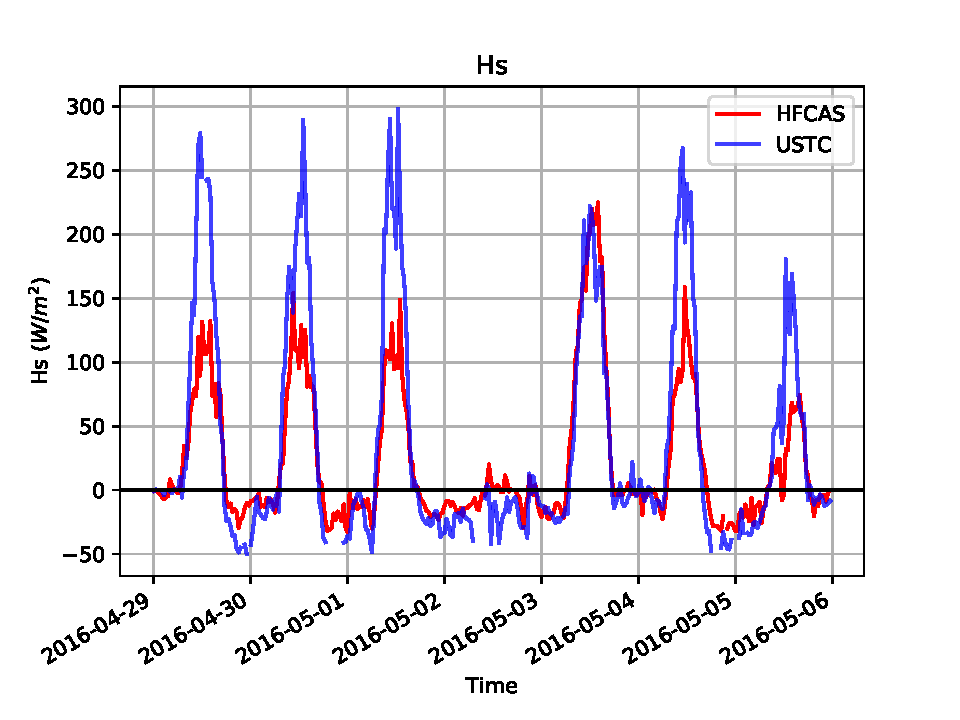
\includegraphics[width=.9\linewidth]{20160429_20160505_Hs}
\caption{2016 年 4 月 29 日至 2016 年 5 月 5 日的感热通量密度}\label{fig:20160429_20160505_Hs}
\note{红色表示科学岛站观测的感热通量密度,蓝色表示中科大站观测的感热通量密度。}
\end{figure}

\section{潜热通量密度}
在一定条件下,加热一个系统,这个系统温度没有发生变化但是发生了相变,
在这种情况下系统中分子之间的相互作用发生了变化而动能没有增加。
这种温度不发生改变但是发生物态变化时吸收或放出的热称为潜热(LE)。
天气系统中常常伴随着物态的变化,尤其是水的三态变化,潜热对能量平衡的影响力不容忽视。\cite{tagkey2006}

图\ref{fig:LE}给出了中科大站与科学岛站两地去除野点之后的潜热通量密度数据,
以 2016 年 2 月 15 日至 2016 年 2 月 19 日这 5 天的潜热通量密度为例,
2 月 15 日至 2 月 18 日均为晴天,2 月 19 日为阴天,从图\ref{fig:20160215_20160219_LE}中可以看出,
无论是中科大站(城市)还是科学岛站(郊区),两地夜间的感热通量密度都比较低,通常不会超过 25\(W/m^2\),
事实上,对全部的潜热通量密度数据进行分析,中科大站的感热通量密度夜晚平均为 8.10 \(W/m^2\),
科学岛站的感热通量密度夜晚平均为 7.28\(W/m^2\),详见表\ref{tab:LE}。
到了白天,潜热通量密度明显上升,正午达到峰值 150\(W/m^2\) 左右,
且白天科学岛站(郊区)的潜热通量密度明显高于中科大站(城市),晴天白天科学岛站比科大站平均高出 29.06 \(W/m^2\)。
阴雨天中科大站与科学岛站两地的潜热通量密度都比较低,和晴天相比,
中科大站阴天的潜热通量密度比晴天平均低 14.96\(W/m^2\),
科学岛站阴天的潜热通量密度比晴天平均低 32.00\(W/m^2\),详见表\ref{tab:LE}。
\begin{figure}[H]
\centering
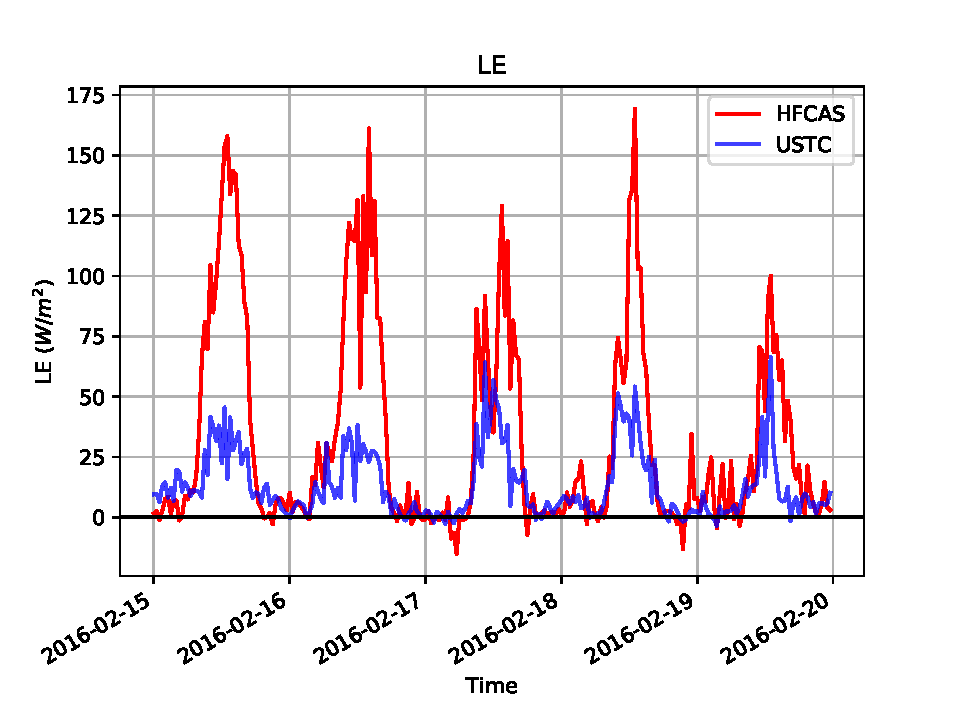
\includegraphics[width=.9\linewidth]{20160215_20160219_LE}
\caption{2016 年 2 月 15 日至 2016 年 2 月 19 日潜热通量密度}\label{fig:20160215_20160219_LE}
\note{红色表示科学岛站观测的潜热通量密度,蓝色表示中科大站观测的潜热通量密度。}
\end{figure}
\begin{table}[H]
\centering
\caption{中科大站与科学岛站潜热通量密度比较}\label{tab:LE}
\begin{tabular}{ccccc}
  \toprule
  & \multicolumn{2}{c}{中科大站} & \multicolumn{2}{c}{科学岛站}\\
  \cmidrule(r){2-3} \cmidrule(r){4-5}
  & 均值 & 标准差 & 均值 & 标准差\\
  \midrule
  全部 & 20.857 & 36.834 & 28.439 & 47.406\\
  晴天 & 31.053 & 44.676 & 46.231 & 61.797\\
  阴天 & 16.096 & 41.126 & 14.233 & 39.429\\
  白天 & 34.418 & 42.185 & 51.607 & 54.671\\
  夜晚 & 8.099 & 24.971 & 7.280 & 25.151\\
  晴天白天 & 54.184 & 51.529 & 83.244 & 66.992\\
  阴天白天 & 20.872 & 41.586 & 22.765 & 42.418\\
  晴天夜晚 & 7.030 & 13.381 & 8.828 & 18.976\\
  阴天夜晚 & 11.929 & 40.278 & 6.881 & 35.054\\
  \bottomrule
\end{tabular}
\note{单位:$W/m^{2}$}
\end{table}
潜热通量密度的变化与水的物态变化密切相关,液态水汽化变成气态水这个过程会吸收能量,
水的多少会直接影响潜热通量密度的大小。科学岛站位于合肥市庐阳区董铺水库科学岛上,
科学岛为西北-东南走向的半岛,被水环绕,水量充足,而中科大站位于合肥市包河区金寨路,四面都是建筑、街道,
处在城市中,水量很少。水量的差异还可以从湿度数据得到反映,如图\ref{fig:20160215_20160219_RH},
相对湿度夜晚通常比较高,2016 年 2 月 15 日至 2016 年 2 月 19 日中科大站测得的相对湿度峰值平均为 51.54\%
而科学岛站的相对湿度夜晚明显高于中科大,这 5 天里科学岛站相对湿度的峰值平均为 81.78\%,比中科大站高出 30.24\%,
到了白天,太阳出来之后相对湿度迅速下降,跌至 30\% 以下。
科学岛站水量更多,使得科学岛站的潜热通量密度相对中科大站更大。
\begin{figure}[H]
\centering
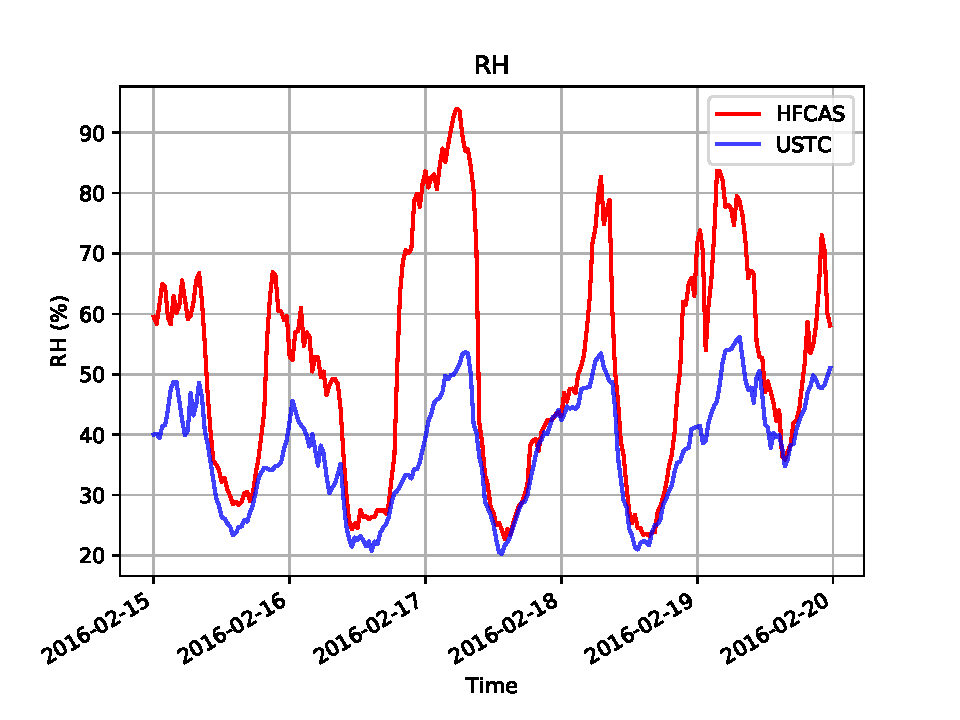
\includegraphics[width=.9\linewidth]{20160215_20160219_RH}
\caption{2016 年 2 月 15 日至 2016 年 2 月 19 日两地相对湿度}\label{fig:20160215_20160219_RH}
\note{图中红色表示科学岛站测得的相对湿度,蓝色表示中科大站测得的相对湿度。}
\end{figure}

\section{城市与郊区的储热}
辐射通量密度、感热通量密度以及潜热通量密度等共同影响着地面的能量平衡,
此外,人类活动产生的人为热,以及向土壤中传导的热也会对能量平衡产生影响,因此下垫面的能量平衡方程可以写为:
\begin{equation}\label{eq:balance}
  R_n + Q = H_s + LE + G_s + \Delta S
\end{equation}
其中 \(R_n\) 为下垫面接收的净辐射通量密度,它可以用向下、向上短波辐射通量密度以及向下、向上长波辐射通量密度这 4 个分量计算得到,见式\ref{eq:Rn},\(Q\) 是由人类活动产生的热通量密度,\(H_s\) 为感热通量密度,\(LE\) 为潜热通量密度,\(G_s\) 是向下传入土壤中的热通量密度,\(\Delta S\) 为空气层内作物或障碍物储存的热通量密度,即城市或郊区的储热。

式\ref{eq:balance}中,\(R_n\)、\(H_s\)、\(LE\) 可以从中科大站与科学岛站的观测数据中直接获取,
向下传入土壤中的热通量密度 \(G_s\) 科学岛站有仪器测量但是中科大站没有,
因此只能忽略这一项,而人类活动产生的热 \(Q\) 不好直接测量,也先将其忽略,
这样便得到:
\begin{equation}\label{eq:simplified_balance}
  R_n = H_s + LE + \Delta S'
\end{equation}
其中 \(\Delta S\) 与 \(\Delta S'\) 的关系如下:
\begin{equation}\label{eq:dS_dS'}
  \Delta S = \Delta S' - G_s + Q
\end{equation}
如果不考虑向下传入土壤中的热通量密度 \(G_s\) 以及人类活动产生的热 \(Q\),那么 \(\Delta S'\) 可以作为 \(\Delta S\) 的近似值,\(\Delta S'\) 可由式\ref{eq:simplified_balance} 计算,结果如图\ref{fig:dS},半月平均值如图\ref{fig:dS_sms},白天夜晚以及不同天气情况的 \(\Delta S'\) 具体可见表\ref{tab:dS}。
\begin{figure}[H]
\centering
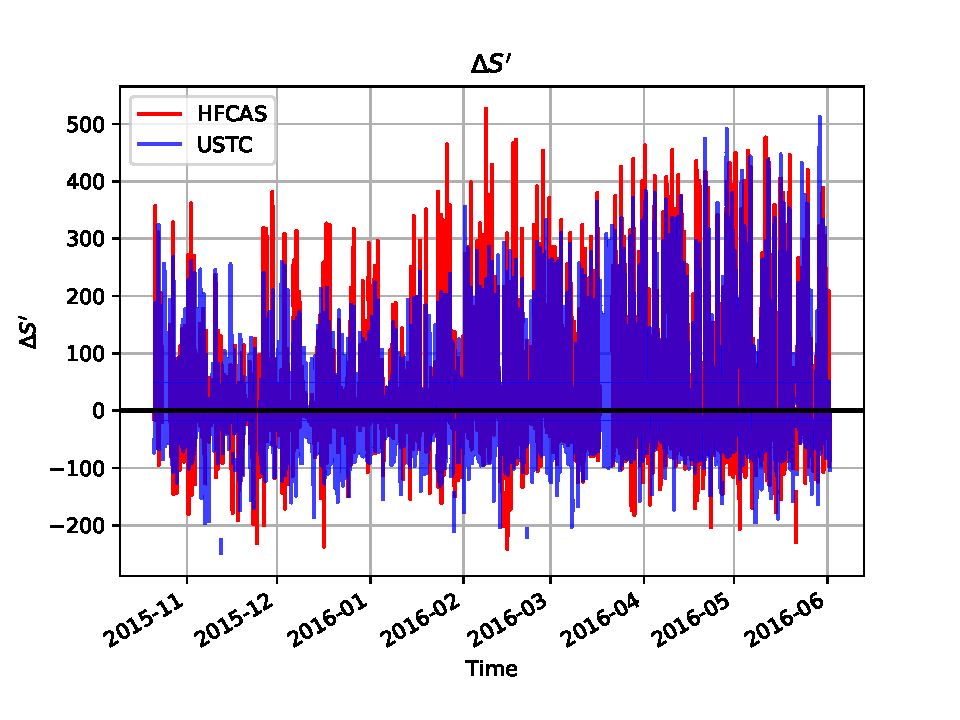
\includegraphics[width=.9\linewidth]{dS}
\caption{城市与郊区的储热}\label{fig:dS}
\note{图中蓝色表示中科大站(城市)的储热,红色表示科学岛站(郊区)的储热。}
\end{figure}
\begin{figure}[H]
\centering
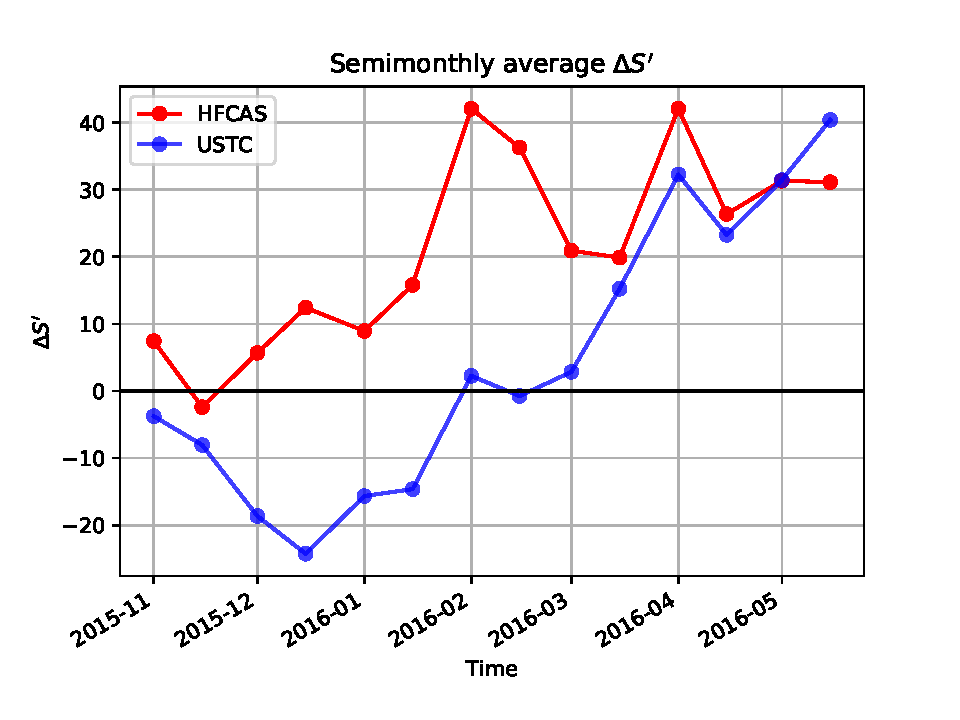
\includegraphics[width=.9\linewidth]{dS_sms}
\caption{城市与郊区储热的半月平均值}\label{fig:dS_sms}
\note{图中蓝色表示中科大站(城市)的储热的半月平均值,红色表示科学岛站(郊区)的储热的半月平均值。}
\end{figure}
\begin{table}[H]
\centering
\caption{中科大站与科学岛站储热通量密度比较}\label{tab:dS}
\begin{tabular}{ccccc}
  \toprule
  & \multicolumn{2}{c}{中科大站} & \multicolumn{2}{c}{科学岛站}\\
  \cmidrule(r){2-3} \cmidrule(r){4-5}
  & 均值 & 标准差 & 均值 & 标准差\\
  \midrule
  全部 & 4.012 & 94.894 & 21.038 & 96.737\\
  晴天 & 22.263 & 122.930 & 49.693 & 139.151\\
  阴天 & -16.767 & 52.446 & -5.944 & 43.269\\
  白天 & 64.269 & 101.833 & 66.513 & 119.802\\
  夜晚 & -52.625 & 33.185 & -20.473 & 34.489\\
  晴天白天 & 107.334 & 119.863 & 133.214 & 152.465\\
  阴天白天 & 5.119 & 54.437 & 2.132 & 47.047\\
  晴天夜晚 & -65.951 & 24.449 & -34.459 & 36.676\\
  阴天夜晚 & -35.890 & 42.214 & -12.895 & 38.418\\
  \bottomrule
\end{tabular}
\note{单位:$W/m^{2}$}
\end{table}
\begin{figure}[H]
\centering
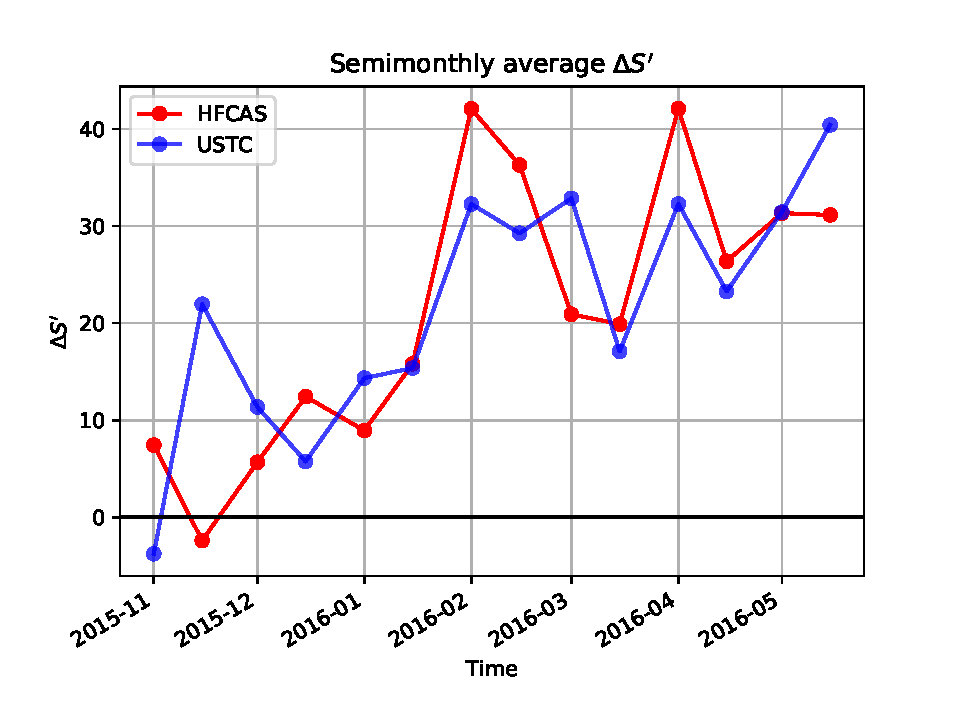
\includegraphics[width=.9\linewidth]{dS_Q}
\caption{城市 (考虑冬季供暖) 与郊区储热的半月平均值}\label{fig:dS_Q}
\note{图中蓝色表示中科大站(城市)的储热的半月平均值,红色表示科学岛站(郊区)的储热的半月平均值,通过对科大的供暖数据进行分析,发现冬季供暖期间会造成 \(30W/m^2\) 的人为热释放,将其叠加至城市的储热中。}
\end{figure}

储热通量密度 \(\Delta S'\) 为正值表示吸热,为负值表示放热,从表\ref{tab:dS}可以看出:晴天平均都是吸热,阴天平均都是放热;白天平均都在吸热,夜晚平均都在放热;晴天白天吸收的热量明显高于阴天白天吸收的热量,晴天夜晚放出的热也要高于阴天夜晚。图\ref{fig:dS_sms}中,中科大站(城市)在 2016 年 2 月之前基本都是负值,之后都是正值,而科学岛站(郊区)观测期间内几乎都是正值,这种现象可能与多种因素有关:首先城市人类活动明显强与郊区,尤其在冬季供暖期间,释放的人为热要比郊区高出不少,供暖期间内(2015 年 11 月 15 日至 2016 年 3 月 15 日),郊区的 \(\Delta S'\) 比城市平均高出 \(29.10W/m^2\),人类活动可能贡献了一部分差异;另外,平衡方程\ref{eq:balance}只考虑了竖直方向的能量收支,并没有考虑水平方向的能量输送,竖直方向的能量不平衡可能是由水平方向的能量输送所造成。

由于没有土壤传输热通量的数据,使用 \(\Delta S'\) 估计 \(\Delta S\) 还是会有一定差异,城市的人类活动比郊区繁忙得多,城市中的人为热也会比郊区高一些,忽略人为热可能会导致计算出的城市储热偏低。为了更准确地计算出城市和郊区的储热,需要添加测量传导到土壤中的热通量的仪器,这些工作有待后续的研究。
